\chapter{ML-KEM}
\label{cap:ml_kem}

    O \ac{ML-KEM} \cite{kyber} é um sistema criptográfico assimétrico baseado na dificuldade de se resolver o problema \ac{MLWE} sobre a estrutura algébrica de reticulados. \ac{ML-KEM} é um dos algoritmos finalistas do programa PQC do \ac{NIST} e selecionado para padronização. Neste capítulo iremos abordar o funcionamento do \ac{ML-KEM}, sua segurança e ataques criptoanalíticos conhecidos contra esse criptossistema. Devido à falta de materiais de fácil compreensão sobre o \ac{ML-KEM} e toda a fundamentação matemática relacionada, este capitulo irá abordar o algoritmo \ac{ML-KEM} de uma maneira mais didática, reduzindo alguns parâmetros e removendo algumas funções que não alteram a estrutura do algoritmo, de forma a simplificar e facilitar o entendimento do leitor.

    O \ac{ML-KEM} é um algoritmo de encapsulamento de chave, e devido à estrutura deste mecanismo é possível separar este criptossistema em duas partes, a parte de cifragem assimétrica, denominada pelo \ac{NIST} como K-PKE, e a parte de encapsulamento de chaves, que seria o próprio \ac{ML-KEM}.

    \section{Esquema de componentes K-PKE}
    \label{sec:k-pke}
    O \ac{ML-KEM} utiliza como subprocesso um conjunto de algoritmos chamado K-PKE, que consiste nos algoritmos de geração de chaves, cifragem e decifragem. No processo de geração de chaves, são geradas as chaves públicas e privadas. Na etapa de cifragem, ocorre a cifragem de uma mensagem de entrada usando as chaves públicas. Por último, na fase de decifragem, é realizada a decifragem de uma mensagem cifrada usando a chave privada.

    Antes de abordar os principais algoritmos do K-PKE, é importante analisar algumas funções que impactam diretamente no seu funcionamento. 
   
    \begin{center}
        $\begin{array}{rl}
            Comprimir_{q}(x,d) &= \lceil (2^d / q) x \rfloor\  \textbf{mod}^{+}\ 2^d,\\
            Descomprimir_{q}(x,d) &= \lceil (q/2^d) x \rfloor
        \end{array}$
    \end{center}

    As funções de comprimir e descomprimir servem para criar uma tolerância de erros durante a cifragem e decifragem de uma mensagem, na qual $x$ é um byte da mensagem, $q$ é o parâmetro estabelecido do \ac{NIST} e $d$ para este caso sempre será o valor 1. A função descomprimir, utilizada na cifragem, é aplicada a cada coeficiente do polinômio que representa uma mensagem cifrada, onde os coeficientes são mantidos em zero caso forem zero ou substituídos por $\lceil q/2^d \rfloor$ se forem 1. A função de comprimir é utilizada para fazer o processo reverso, em que se o coeficiente for mais próximo de $\lceil q/2^d \rfloor$ do que de zero, retorna um, caso contrário retorna zero. 

    \begin{algorithm}[!htbp]
        \SetAlgoLined
        \Entrada{Vetor de bytes $B = b_0,b_1,...,b_{64\eta - 1}$}
        \Saida{Um polinômio $f \in \mathbb{Z}_{q}{[}x{]}/ \langle x^n + 1 \rangle$}
        \Para{$i \leftarrow 0$ até $n-1$}{
            $a \leftarrow_{aleat\acute{o}rio} {[} 0, \eta {]}$\\
            $b \leftarrow_{aleat\acute{o}rio} {[} 0, \eta {]}$\\
            $f_i \leftarrow a - b$
        }
        
        \Retorna{$f_{0} + f_{1} x + f_{2} x^{2} + ... + f_{n-1} x^{n-1}$}
    
        \caption{Distribuição Binomial Centrada}
        \label{algo:cbd}
    \end{algorithm}
    
    O Algoritmo \ref{algo:cbd} retorna um polinômio de grau $n$ com os coeficientes baseados na distribuição binomial centrada. A distribuição binomial centrada neste caso é uma distribuição de probabilidade com centro em zero, como ilustra a Figura \ref{fig:cbd}. Note que os coeficientes do polinômio resultante do Algoritmo \ref{algo:cbd} podem assumir apenas os valores no intervalo ${[}-\eta,\eta{]}$, dessa forma, este algoritmo é utilizado para gerar vetores de grau pequeno. 

    \begin{figure}[htb!]
        \centering
        \caption{Distribuição binomial discreta centrada em 0.}
        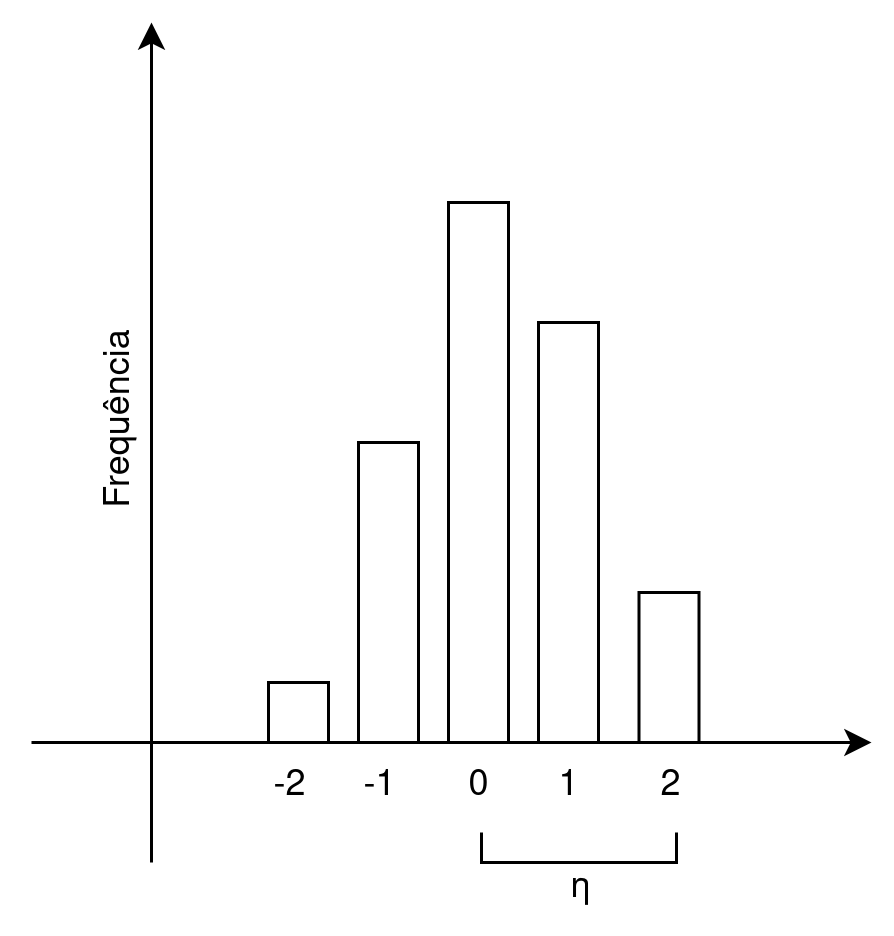
\includegraphics[width=0.65\textwidth]{Figuras/cbd.png}\\
        \footnotesize{Fonte: O autor.}
        \label{fig:cbd}
    \end{figure}

    Como pode ser visto na Figura \ref{fig:kyber_key_gen}, a geração de chaves consiste em gerar quatro matrizes de polinômios, sendo as matrizes \textbf{A} e \textbf{t} as chaves públicas, a matriz \textbf{s} a chave privada e a matriz \textbf{e} apenas uma matriz aleatória de perturbação que pode ser descartada após o final da operação. Perceba que no Algoritmo \ref{algo:kyber_keygen} a ordem das matrizes estão em função do parâmetro k, e seus elementos são polinômios de grau 256 com coeficientes pertencentes ao intervalo ${[}0,3329{]}$. Os elementos da matriz \textbf{A} devem ser gerados o mais aleatório possível, enquanto os elementos das matrizes \textbf{s} e \textbf{e} devem ser gerados por uma distribuição de probabilidade binomial centrada em zero pelo Algoritmo \ref{algo:cbd}. Segundo \cite{kyber}, a motivação para a escolha desta distribuição foi para dificultar alguns ataques conhecidos a esquemas baseados no \ac{LWE}. O Algoritmo \ref{algo:kyber_keygen} representa este processo de geração de chaves.

    \begin{figure}[htb!]
        \centering
        \caption{Ilustração da geração de chaves do K-PKE no modelo matricial.}
        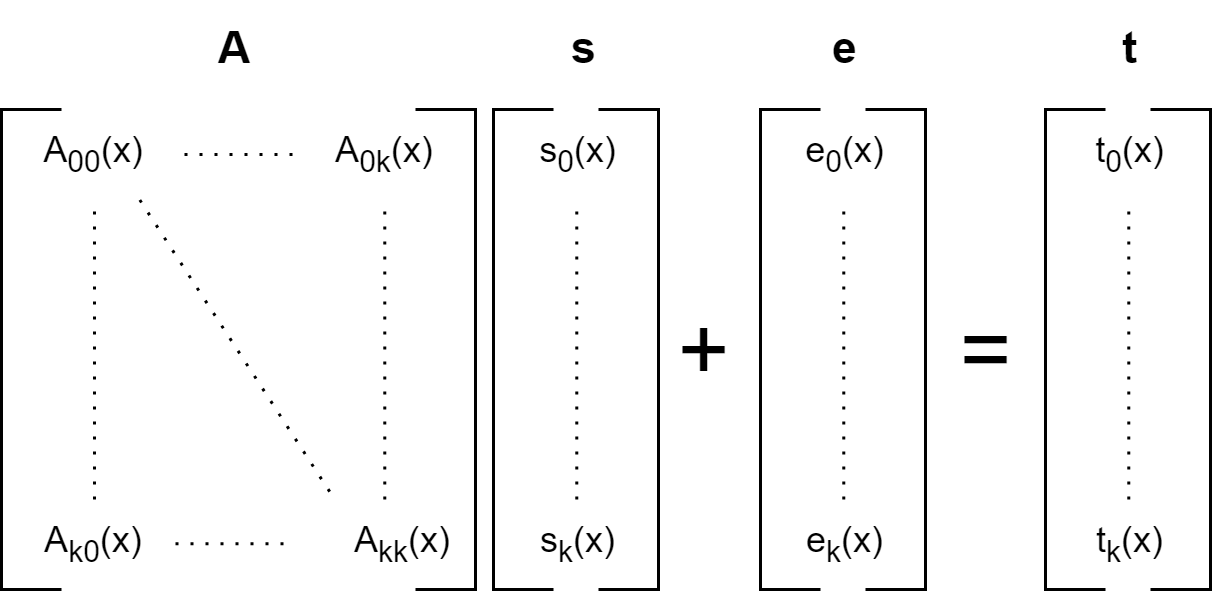
\includegraphics[width=0.75\textwidth]{Figuras/kyber_keygen.png}\\
        \footnotesize{Fonte: O autor.}
        \label{fig:kyber_key_gen}
    \end{figure}

    \begin{algorithm}[!htbp]
        \SetAlgoLined
        \Saida{Chave privada $s \in {[}\mathbb{Z}_{q}{[}x{]}/ \langle x^n + 1 \rangle{]}^k$}
        \Saida{Chave pública $t \in {[}\mathbb{Z}_{q}{[}x{]}/ \langle x^n + 1 \rangle{]}^k$}
        \Saida{Chave pública $A \in {[}\mathbb{Z}_{q}{[}x{]}/ \langle x^n + 1 \rangle{]}^{k \times k}$}
        
        \Para{$i \leftarrow 0$ até $k - 1$}{
            \Para{$j \leftarrow 0$ até $k - 1$}{
                A[i][j] $\leftarrow$ random\_poly()\\
            }
        }

        \Para{$i \leftarrow 0$ até $k - 1$}{
            s[i] $\leftarrow$ random\_poly\_cbd($\eta_1$)\\
        }

        \Para{$i \leftarrow 0$ até $k - 1$}{
            e[i] $\leftarrow$ random\_poly\_cbd($\eta_1$)\\
        }

        $t \leftarrow As + e$\\
        
        \Retorna{s,t,A}
    
        \caption{K-PKE - Geração de chaves}
        \label{algo:kyber_keygen}
    \end{algorithm}

    A cifragem de uma mensagem conforme ilustra a Figura \ref{fig:kyber_enc} consiste na geração de uma matriz \textbf{u} e um polinômio v, isto é, uma mensagem cifrada pelo K-PKE será representada por estes dois elementos. O processo de cifragem de uma mensagem M, representada por um polinômio, consiste em calcular a transposta das chaves públicas \textbf{A} e \textbf{t}, gerar duas matrizes e um polinômio de forma aleatória que seguem a distribuição binomial centrada em zero, e computar a matriz \textbf{u} e o polinômio v como indica o Algoritmo \ref{algo:kyber_encryption}.

    \begin{figure}[htb!]
        \centering
        \caption{Ilustração da cifragem de uma mensagem usando K-PKE no modelo matricial.}
        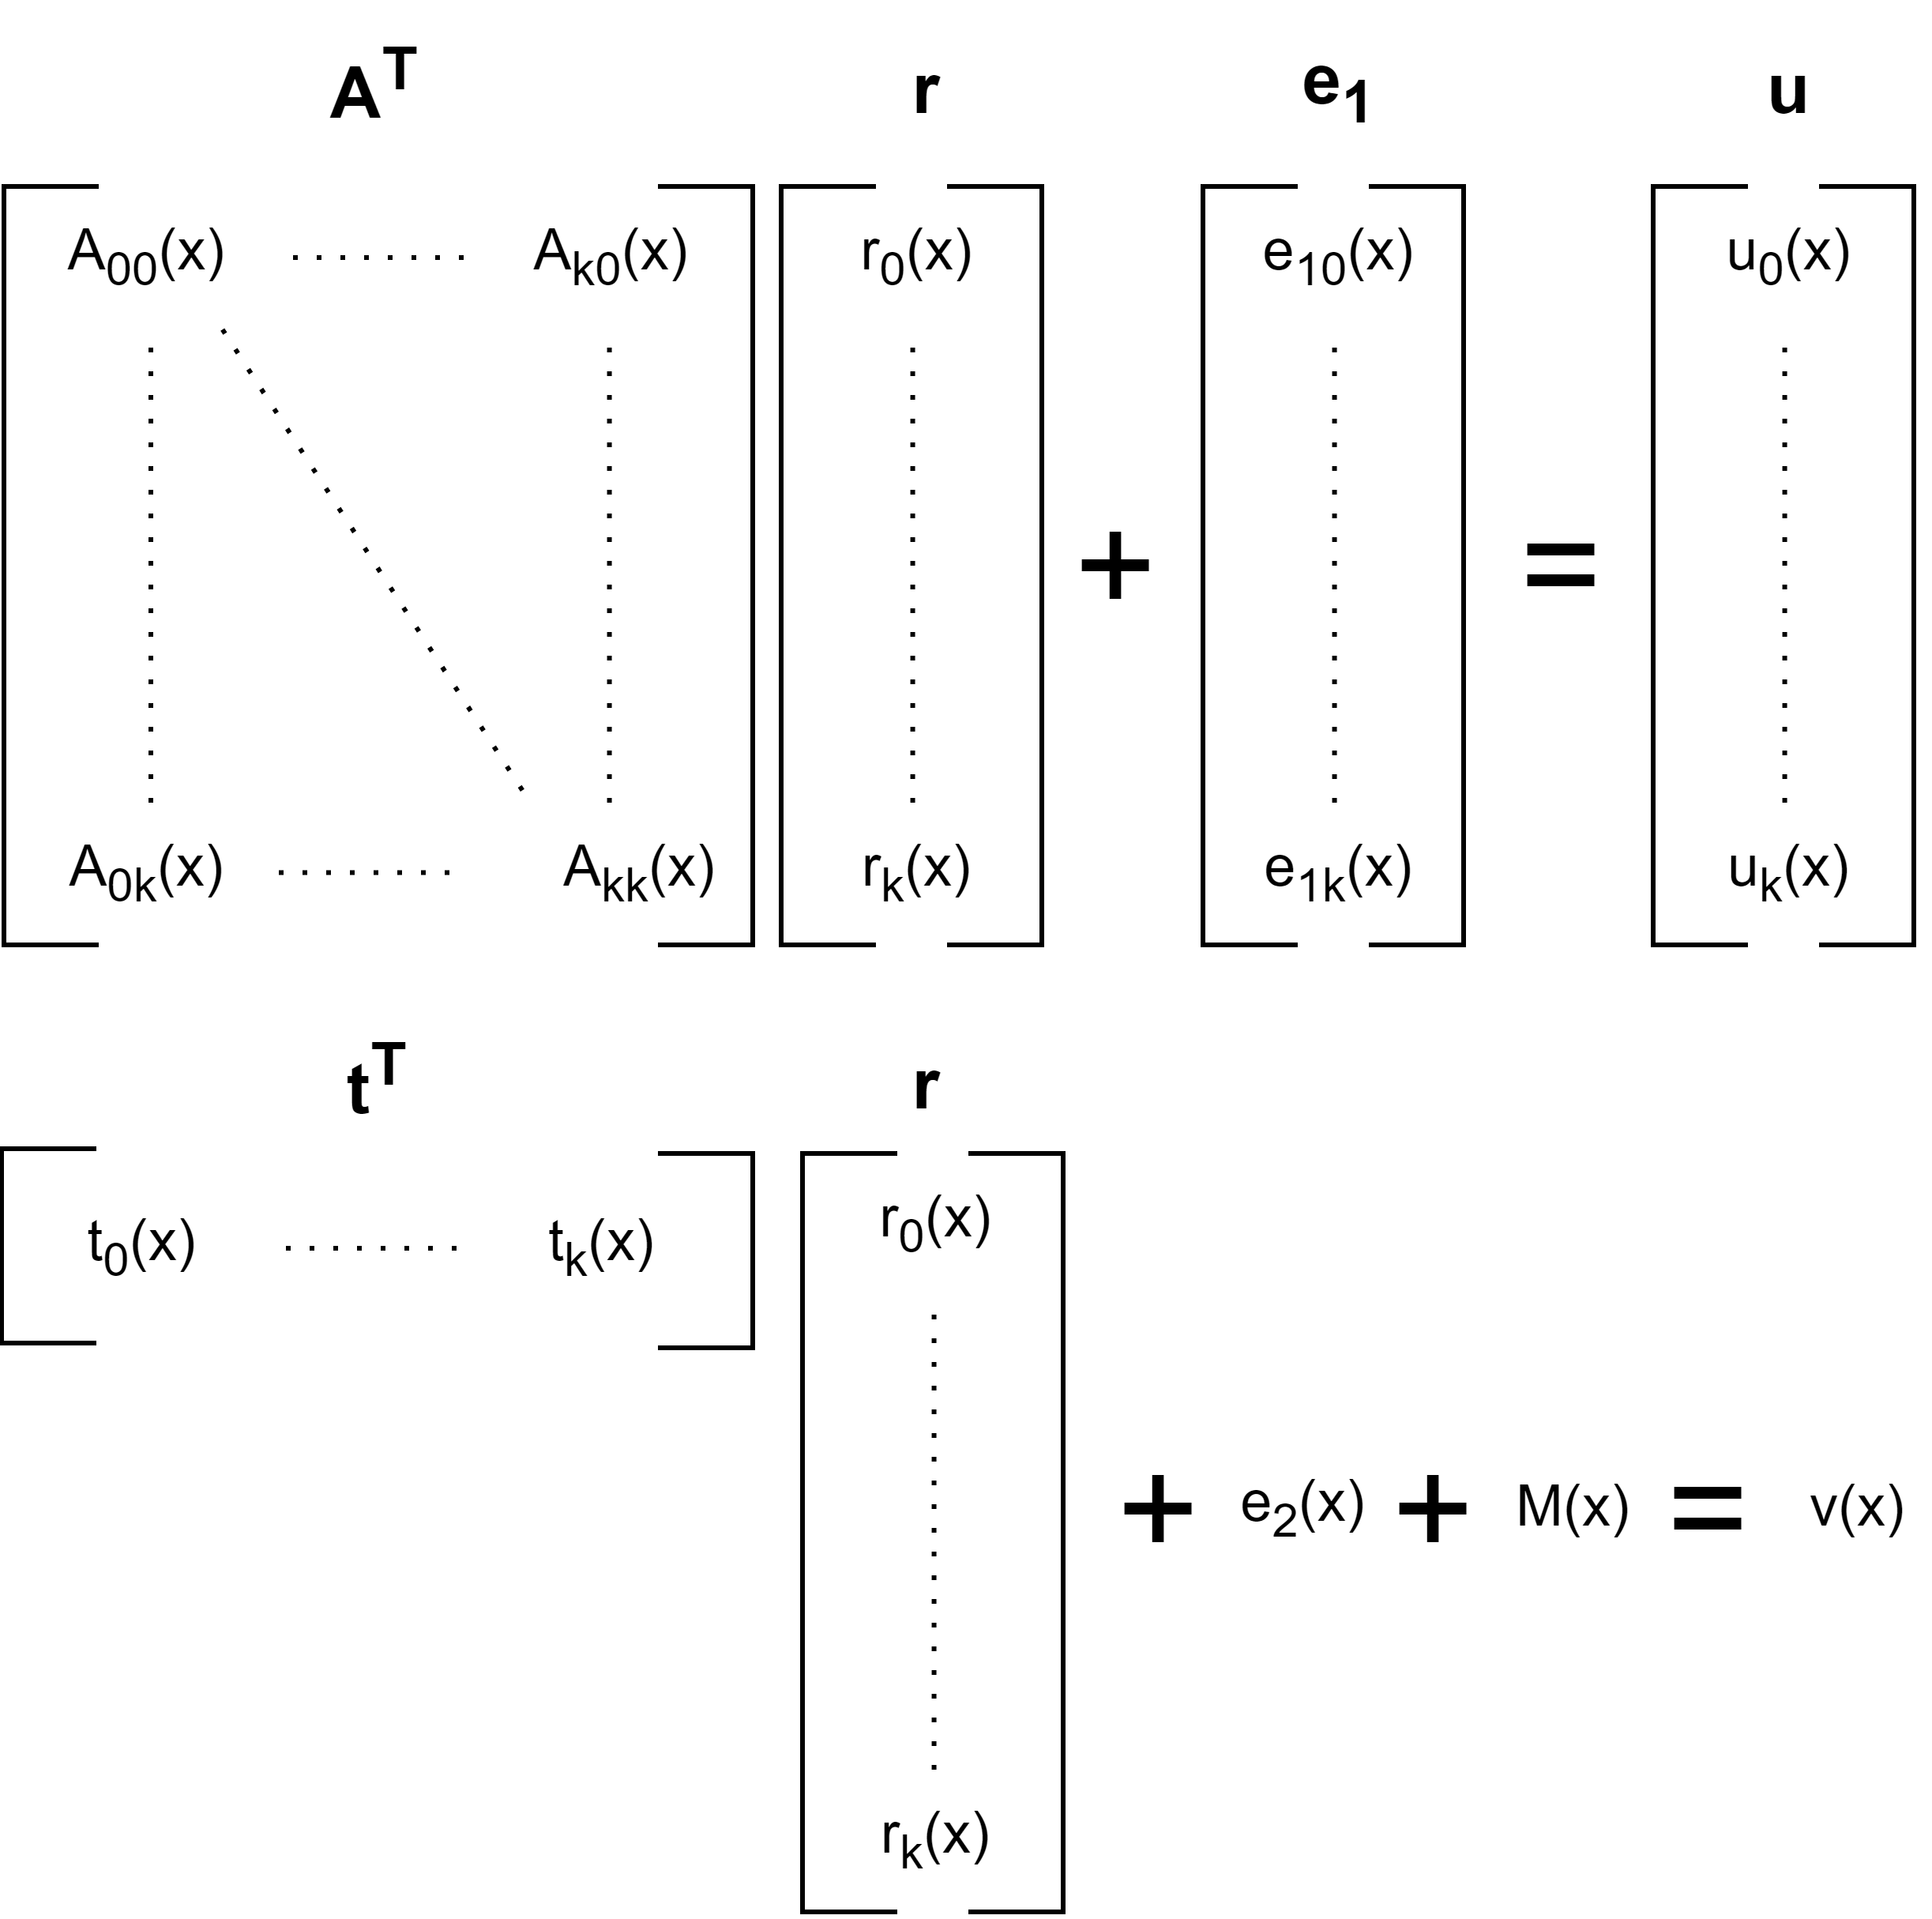
\includegraphics[width=0.75\textwidth]{Figuras/kyber_enc.png}\\         
        \footnotesize{Fonte: O autor.}
        \label{fig:kyber_enc}
    \end{figure}

    \begin{algorithm}[!htbp]
        \SetAlgoLined
        \Entrada{Chave pública A}
        \Entrada{Chave pública t}
        \Entrada{Mensagem m de 32 bytes}
        \Saida{Texto cifrado $u \in {[}\mathbb{Z}_{q}{[}x{]}/ \langle x^n + 1 \rangle{]}^k$}
        \Saida{Texto cifrado $v \in \mathbb{Z}_{q}{[}x{]}/ \langle x^n + 1 \rangle$}
   
        $A^T   \leftarrow CalculaTransposta(A, k)$\\
        $t^{T} \leftarrow CalculaTransposta(t, k)$\\
        
        \Para{$i \leftarrow 0$ até $k - 1$}{
            r[i] $\leftarrow$ random\_poly\_cbd($\eta_1$)\\
        }

        \Para{$i \leftarrow 0$ até $k - 1$}{
            $e_1$[i] $\leftarrow$ random\_poly\_cbd($\eta_2$)\\
        }

        $e_2 \leftarrow$ random\_poly\_cbd($\eta_2$)\\

        $u \leftarrow A^{T} r + e_{1}$\\
        $v \leftarrow t^{T} r + e_{2} + Descomprimir_{q}(m,1)$\\
        
        \Retorna{u,v}
    
        \caption{K-PKE - Cifragem}
        \label{algo:kyber_encryption}
    \end{algorithm}

    A decifragem do K-PKE é relativamente simples, como pode ser visto na Figura \ref{fig:kyber_dec}, basta calcular a transposta da chave privada \textbf{s}, computar $m' = v - s^T u$ e aplicar a função de comprimir em $m'$ conforme o Algoritmo \ref{algo:kyber_decryption}.

    \begin{figure}[htb!]
        \centering
        \caption{Ilustração da decifragem de uma mensagem usando K-PKE no modelo matricial.}
        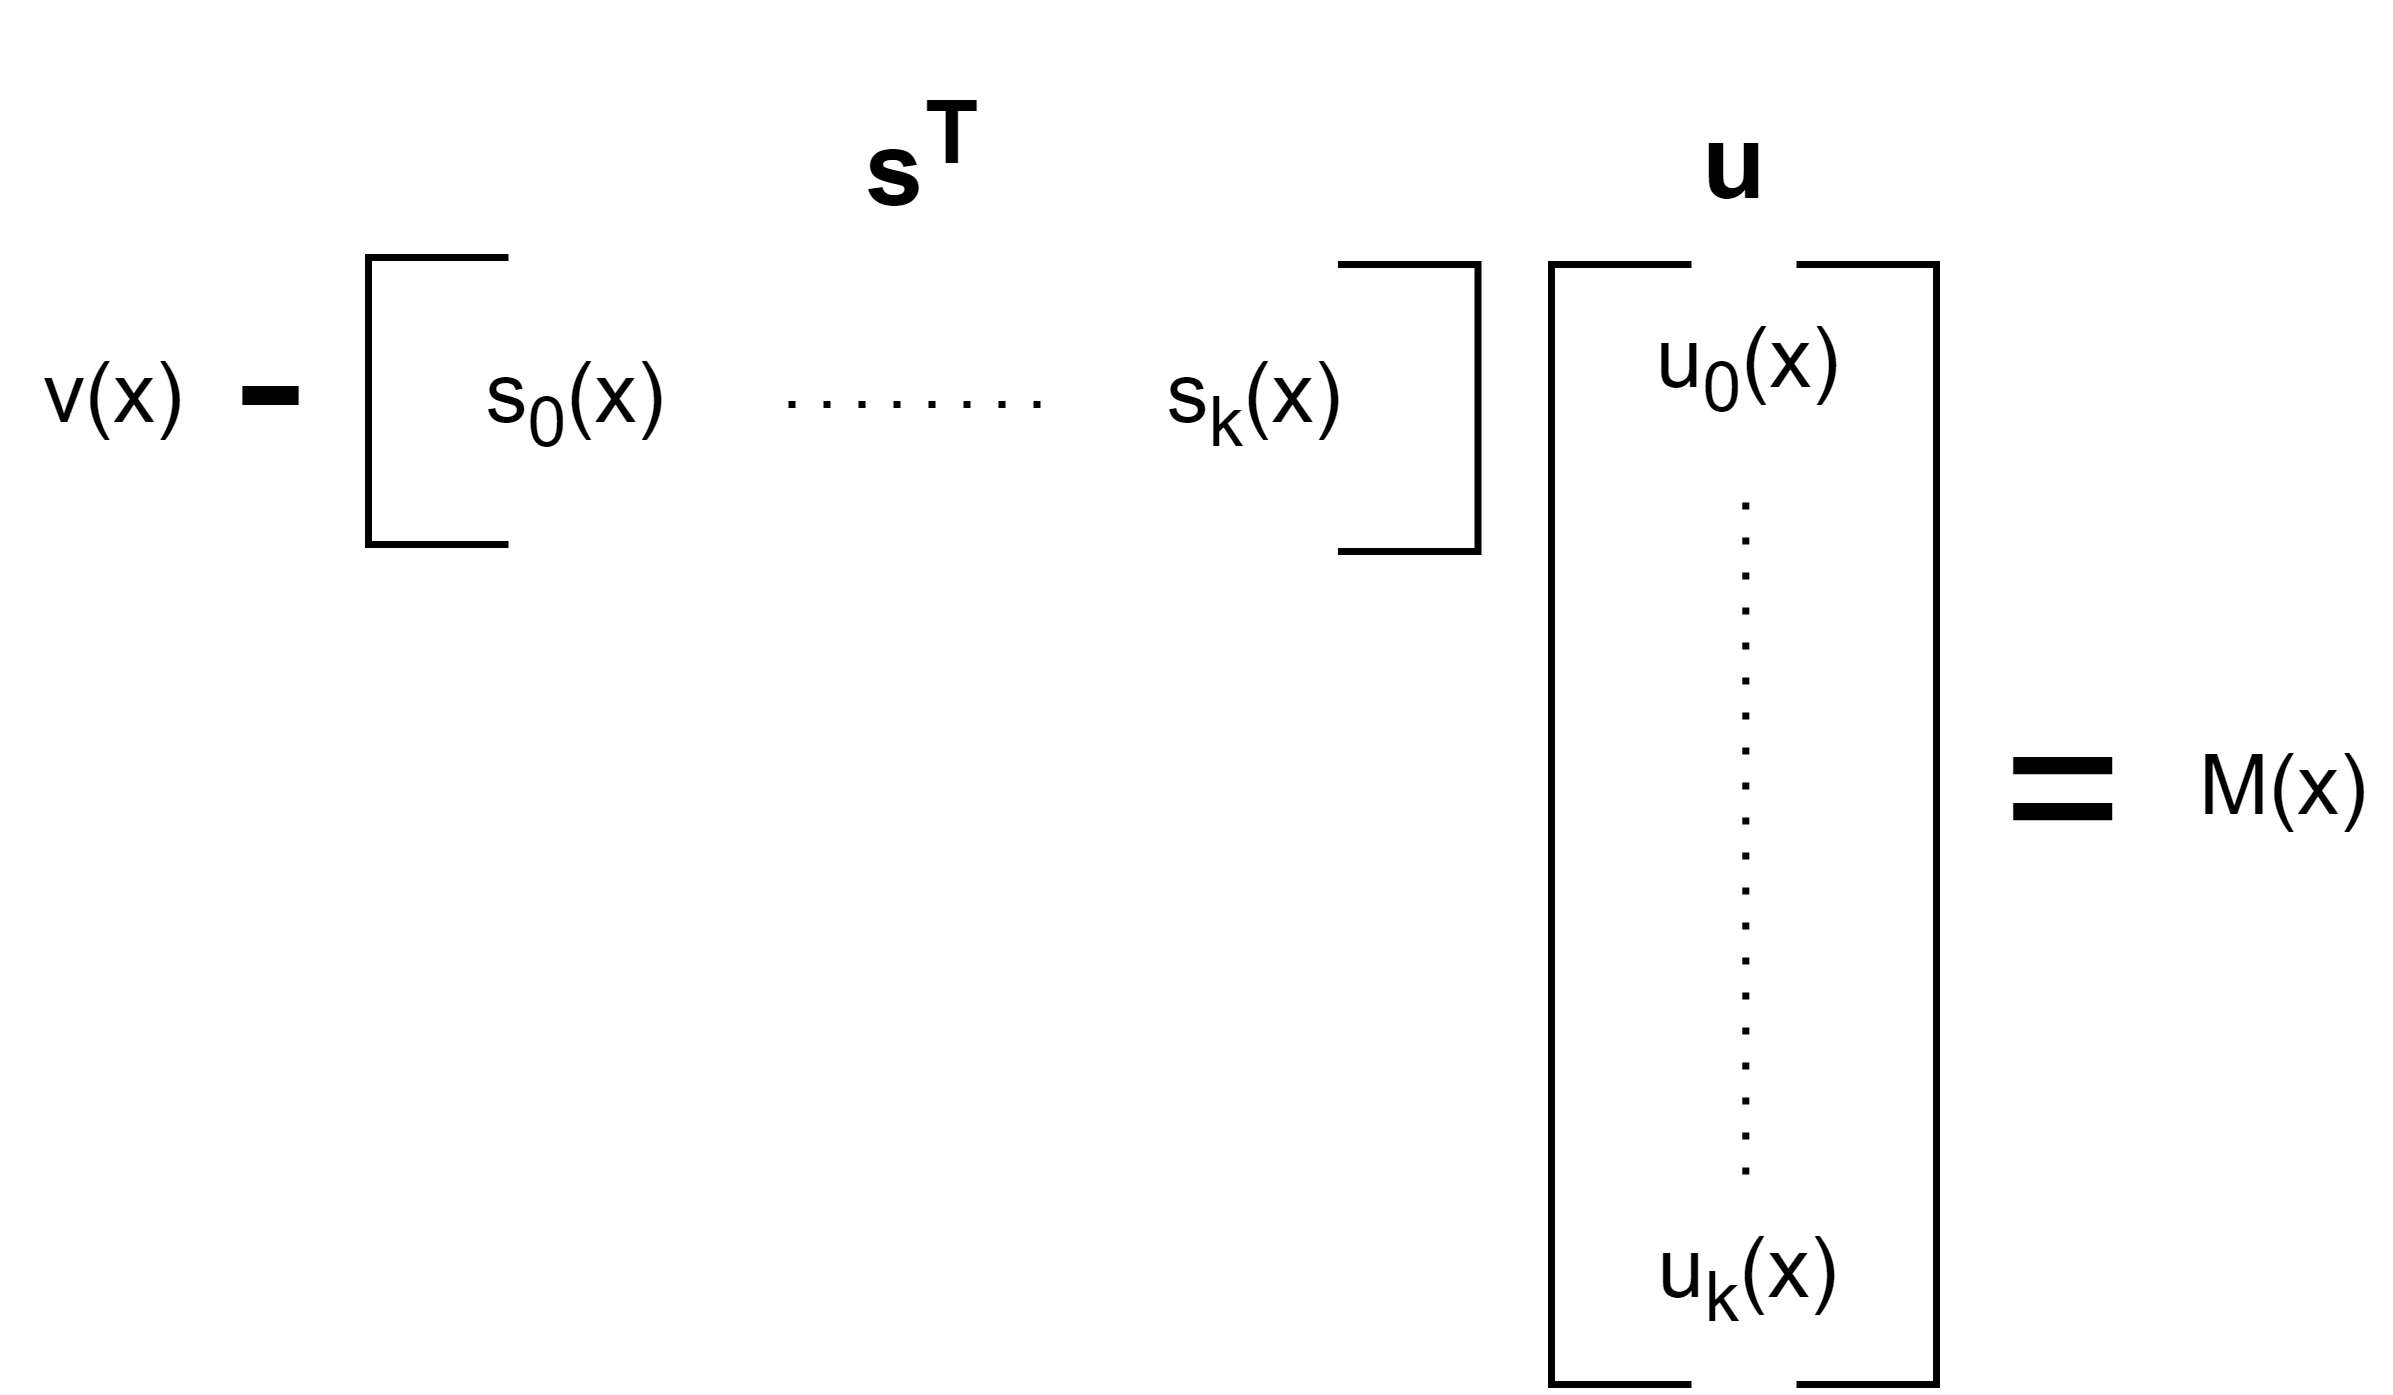
\includegraphics[width=0.65\textwidth]{Figuras/kyber_dec.png}\\
        \footnotesize{Fonte: O autor.}
        \label{fig:kyber_dec}
    \end{figure}

    \begin{algorithm}[!htbp]
            \SetAlgoLined
            \Entrada{Chave privada s}
            \Entrada{Texto cifrado $u \in {[}\mathbb{Z}_{q}{[}x{]}/ \langle x^n + 1 \rangle{]}^k$}
            \Entrada{Texto cifrado $v \in \mathbb{Z}_{q}{[}x{]}/ \langle x^n + 1 \rangle$}
            \Saida{Mensagem m de 32 bytes}
            
            $s^T = CalculaTransposta(s, k)$\\
            $m' = v-s^T u$\\
            $m = Comprimir_{q}(m',1)$
            
            \Retorna{m}
        
            \caption{K-PKE - Decifragem}
            \label{algo:kyber_decryption}
        \end{algorithm}

    Para entender o porquê deste processo de cifragem e decifragem funcionar, observe a seguinte derivação da equação de decifragem do Algoritmo \ref{algo:kyber_decryption}.

    \begin{center}
        $\begin{array}{c}
            v-s^{T}u\\
            (t^{T}r + e_2 + \lceil q/2 \rfloor M) - (s^T(A^T r + e_1))\\
            ((As + e)^T r + e_2 + \lceil q/2 \rfloor M) - (s^T(A^T r + e_1))\\
            ((As)^T r + e^T r + e_2 + \lceil q/2 \rfloor M) - (s^T A^T r + s^T e_1)\\
            (s^T A^T r + e^T r + e_2 + \lceil q/2 \rfloor M) - (s^T A^T r + s^T e_1)\\
            \lceil q/2 \rfloor M + e^T r + e_2 - s^T e_1\\
        \end{array}$
    \end{center}

    Perceba que a função Descomprimir multiplica cada byte da mensagem M(x) por $q / 2$ no processo de cifragem, e depois são adicionados ruídos de norma pequena. Na última linha da derivação temos uma mensagem M com coeficientes grandes adicionado de ruídos com norma pequena, uma vez que foram gerados seguindo uma distribuição de probabilidade centrada em zero. Desta forma é possível remover os ruídos realizando um arredondamento através da função Comprimir.

    Segue um exemplo prático das três etapas do K-PKE com os parâmetros ajustados em $n = 4$, $k = 2$, $q = 3329$, $\eta_1 = 2$ e $\eta_2 = 2$, para simplificar o processo.

    \noindent
    \textbf{Geração de chaves}

        O primeiro passo é gerar a matriz \textbf{A} que será uma das chaves públicas, a matriz \textbf{A} neste caso é uma matriz $2 \times 2$, então é necessário gerar quatro polinômios de grau 3 com coeficientes entre 0 e 3329. Os coeficientes devem ser o mais aleatório possível.
        
        \begin{center}
            \textbf{A} = $\begin{bmatrix}
               2791 + 1035 x + 1916 x^2 + 339 x^3  & 2154 + 2311 x + 517 x^2 + 2496 x^3 \\
               632 + 3048 x + 416 x^2 + 930 x^3  & 1029 + 699 x + 1587 x^2 + 524 x^3
            \end{bmatrix}$
        \end{center}
        

        Para gerar a matriz \textbf{s} e a matriz \textbf{e} é necessário gerar uma matriz coluna $2 \times 1$ com polinômios de grau 3 e com coeficientes entre -2 e 2. Segundo a distribuição binomial centrada em zero, os polinômios de \textbf{s} devem ter mais coeficientes próximos à 0.

        \begin{center}
            \textbf{s} = $\begin{bmatrix}
               -2 x + x^2 + x^3  \\
                1 - 1 x + -2 x^2 - 1 x^3
            \end{bmatrix}$
            %
            \textbf{e} = $\begin{bmatrix}
                1 + 1 x + 2 x^3 \\
                -1 -1 x + 1 x^2 -1 x^3
            \end{bmatrix}$
        \end{center}

        Por fim, para gerar a chave pública \textbf{t}, deve-se computar t = \textbf{A} \textbf{s} + \textbf{e}.

        \begin{center}
             \textbf{t} = $\begin{bmatrix}
                2394 + 1159 x + 105 x^2 + 1857 x^3 \\
                492 + 3023 x + 2948 x^2 + 2686 x^3 
            \end{bmatrix}$   
        \end{center}

        Deve-se ter cuidado ao realizar as operações entre polinômios, pois estes elementos pertencem ao anel quociente $\mathbb{Z}_{3329}[x] / \langle x^4+1 \rangle$. Um exemplo de como trabalhar com as operações de soma, subtração e multiplicação pode ser conferida no Apêndice \ref{ap:abstract_algebra} nos Exemplos \ref{exemplo:soma_em_Z[x]/<I>} e \ref{exemplo:multiplicacao_em_Z[x]/<I>}.

    \noindent
    \textbf{Cifragem}

    Seja M  = 1101 uma mensagem que deseja-se cifrar com K-PKE, representada pelo polinômio M(x) = $1 + 1x + 0 x^2 + 1x^3 = 1+x+x^3$. Primeiro deve-se calcular a transposta das matrizes \textbf{A} e \textbf{t}.

    \begin{center}
       $\textbf{A}^T$ = $\begin{bmatrix}
           2791 + 1035 x + 1916 x^2 + 339 x^3  & 632 + 3048 x + 416 x^2 + 930 x^3 \\
           2154 + 2311 x + 517 x^2 + 2496 x^3  & 1029 + 699 x + 1587 x^2 + 524 x^3
        \end{bmatrix}$

       $\textbf{t}^T$ = $\begin{bmatrix}
           2394 + 1159 x + 105 x^2 + 1857 x^3 & 492 + 3023 x + 2948 x^2 + 2686 x^3 
        \end{bmatrix}$
    \end{center}

    O próximo passo é gerar as matrizes de ruído aleatório \textbf{r} e \textbf{$e_1$}, e o polinômio de ruído \textbf{$e_2$}.

    \begin{center}
        \textbf{r} = $\begin{bmatrix}
           -1 + x + x^2 + 2 x^3 \\
            1 + x^3
        \end{bmatrix}$
        %
        $\textbf{e}_1$ = $\begin{bmatrix}
            1 + x + x^2 \\
            -1 -x + x^2 -x^3
        \end{bmatrix}$
        %
        $e_2(x) = -x^2 + x^3$
    \end{center}

    A cifragem de uma mensagem M(x) gera dois elementos, uma matriz \textbf{u} e um polinômio v(x). A geração da matriz \textbf{u} é obtida computando $\textbf{A}^T \textbf{r} + \textbf{e}_1$, o resultado desta operação segue abaixo. 

    
    \begin{center}
        \textbf{u} = $\begin{bmatrix}
            246 + 218 x + 719 x^2 + 3098 x^3 \\
            527 + 2082 x + 20 x^2 + 2863 x^3
        \end{bmatrix}$
    \end{center}

    Antes de realizar o cálculo de v(x) é preciso aplicar a função Descomprimir a mensagem M(x), que consiste em multiplicar cada coeficiente da mensagem M(x) por $q/2^d$ e arredondar para o inteiro mais próximo. Segundo a documentação do \ac{NIST} os parâmetros q e d da função Descomprimir são respectivamente 3329 e 1. Desta forma, a mensagem M(x) passa a ser $M(x) = 1665 + 1665x + 1665 x^3$. Com isso, para obtermos o último elemento da mensagem cifrada, o polinômio v(x), deve-se computar $\textbf{t}^T$ \textbf{r} + $e_2$(x) + M(x).

    \begin{center}
        $v(x) = 2447 + 908 x + 3323 x^2 + 2381 x^3$
    \end{center}

    \noindent
    \textbf{Decifragem}

    Para realizar a decifragem de \textbf{u} e v(x), é necessário calcular a transposta da chave privada \textbf{s} e computar $m'(x) = v - \textbf{s}^T u$, após computado $m'(x)$ deve-se aplicar a função Comprimir a ela para realizar o arredondamento, assim obtendo a mensagem original M(x). 

    \begin{center}
            $\textbf{s}^T$ = $\begin{bmatrix}
               -2 x + x^2 + x^3 & 1 - 1 x + -2 x^2 - 1 x^3
            \end{bmatrix}$
    \end{center}
    
    \begin{center}
            $m'(x) = 2447 + 908 x + 3323 x^2 + 2381 x^3 -$
            
            $\begin{bmatrix}
               -2 x + x^2 + x^3 & 1 - 1 x + -2 x^2 - 1 x^3
            \end{bmatrix}$
            %
            $\begin{bmatrix}
            246 + 218 x + 719 x^2 + 3098 x^3 \\
            527 + 2082 x + 20 x^2 + 2863 x^3
        \end{bmatrix}$
    \end{center}

    \begin{center}
        $m'(x) = 1663 + 1245 x + 206 x^2 + 1874 x^3$
    \end{center}

    Aplicando a função Comprimir em m'(x), obtemos a mensagem original M, finalizando o processo de decifragem do K-PKE.

    \begin{center}
        $M(x) = 1 + 1 x + 0 x^2 + 1 x^3$ \\
        $M = 1101$
    \end{center}
    
    %https://link.springer.com/chapter/10.1007/978-981-19-7644-5_4
    %https://www.youtube.com/watch?v=94fdZvSx-NY&t=429s ******** IMPORTANTE  *********
    %https://asecuritysite.com/encryption/lwe3

\section{Encapsulamento de chaves ML-KEM}
\label{sec:ml-kem}
    O \ac{ML-KEM} é um algoritmo de encapsulamento de chave, ou seja, como dito na Seção \ref{sec:kem}, os algoritmos de encapsulamento de chave têm como objetivo estabelecer uma chave simétrica aleatória em comum entre duas partes. A principal diferença entre o \ac{ML-KEM} e o K-PKE, está na mensagem cifrada, enquanto o K-PKE permite cifrar uma mensagem qualquer, o \ac{ML-KEM} determina a mensagem cifrada, esta mensagem é a chave simétrica compartilhada. A nomenclatura de alguns termos também é diferente, as chaves públicas são chamadas de chaves de encapsulamento, a chave privada é dita de desencapsulamento.

    O funcionamento do \ac{ML-KEM} é semelhante ao K-PKE, entretanto a forma como essa comunicação deve ocorrer é pré-estabelecida, e deve seguir o diagrama da Figura \ref{fig:kem_nist} segundo o \ac{NIST}. Perceba que não são cifradas e decifradas mensagens quaisquer como no K-PKE. Em vez disso, o algoritmo gera esta mensagem que é a chave simétrica compartilhada de forma aleatória. A razão disso se dá pelo fato do \ac{ML-KEM} ser um algoritmo de encapsulamento de chave, este abordado no Capítulo \ref{cap:criptografia}.

    \begin{figure}[htb!]
        \centering
        \caption{Estabelecimento de uma chave compartilhada com o \ac{ML-KEM}.}
        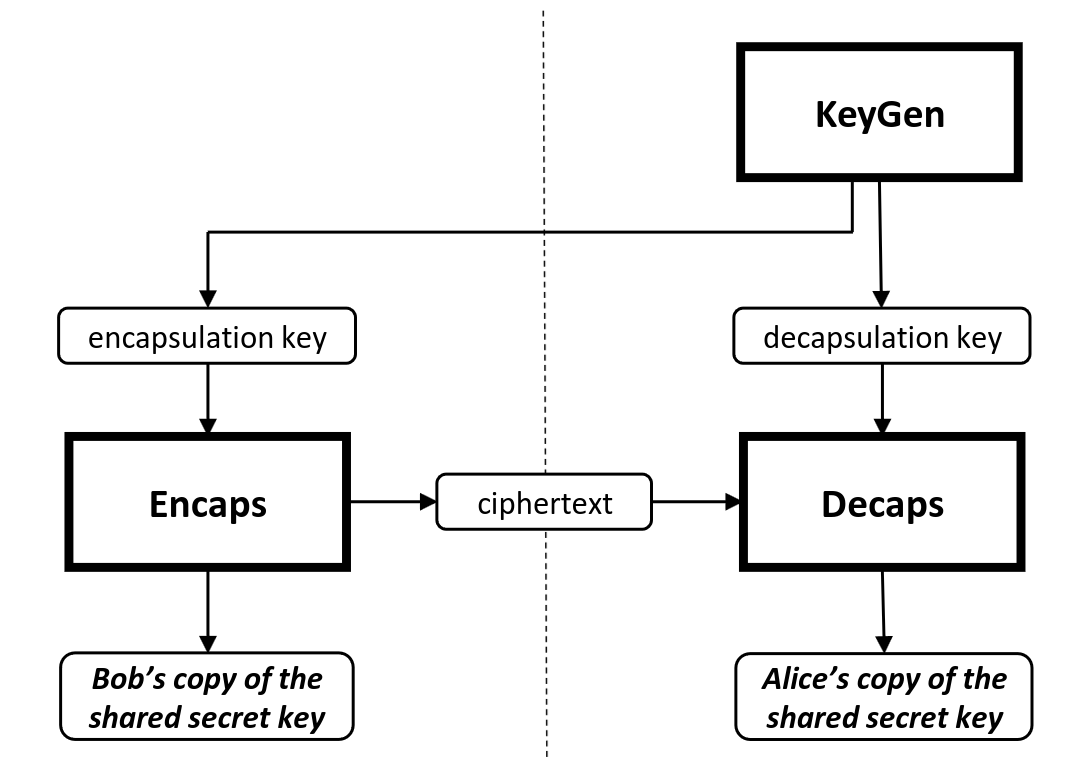
\includegraphics[width=0.75\textwidth]{Figuras/kem_nist.png}\\
        \footnotesize{Fonte: \cite{kyber}.}
        \label{fig:kem_nist}
    \end{figure}

    \begin{algorithm}[!htbp]
            \SetAlgoLined
            \Saida{Chave de desencapsulamento $dk\_pke\_s \in {[}\mathbb{Z}_{q}{[}x{]}/ \langle x^n + 1 \rangle{]}^k$}
            \Saida{Chave de encapsulamento $ek\_pke\_t \in {[}\mathbb{Z}_{q}{[}x{]}/ \langle x^n + 1 \rangle{]}^k$}
            \Saida{Chave de encapsulamento $ek\_pke\_a \in {[}\mathbb{Z}_{q}{[}x{]}/ \langle x^n + 1 \rangle{]}^{k \times k}$}
            
            k\_pke\_s, k\_pke\_t, k\_pke\_a $\leftarrow$ k\_pke\_keygen()\\
            dk\_pke\_s $\leftarrow$ k\_pke\_s\\
            ek\_pke\_t $\leftarrow$ k\_pke\_t\\
            ek\_pke\_a $\leftarrow$ k\_pke\_a
            
            \Retorna{dk\_pke\_s, ek\_pke\_t, ek\_pke\_a}
        
            \caption{ML-KEM - Geração de chaves}
            \label{algo:ml_kem_keygen}
        \end{algorithm}

        No modelo simplificado da geração de chaves do \ac{ML-KEM}, descrito pelo Algoritmo \ref{algo:ml_kem_keygen}, a geração de chaves é idêntica à geração de chaves do K-PKE, com apenas algumas renomeações nas chaves criptográficas, em que dk\_pke\_s é a chave privada de desencapsulamento, ek\_pke\_t e ek\_pke\_a são as chaves públicas de encapsulamento.
        
        \begin{algorithm}[!htbp]
            \SetAlgoLined
            \Entrada{Chave de encapsulamento $ek\_pke\_t \in {[}\mathbb{Z}_{q}{[}x{]}/ \langle x^n + 1 \rangle{]}^k$}
            \Entrada{Chave de encapsulamento $ek\_pke\_a \in {[}\mathbb{Z}_{q}{[}x{]}/ \langle x^n + 1 \rangle{]}^{k \times k}$}
            \Saida{Chave compartilhada cifrada $c\_u \in {[}\mathbb{Z}_{q}{[}x{]}/ \langle x^n + 1 \rangle{]}^k$}
            \Saida{Chave compartilhada cifrada $c\_v \in {[}\mathbb{Z}_{q}{[}x{]}/ \langle x^n + 1 \rangle{]}^k$}
            \Saida{Chave compartilhada $K \in \mathbb{Z}_{q}{[}x{]}/ \langle x^n + 1 \rangle$}
       
            K $\leftarrow$ random\_poly()\\
            c\_u, c\_v $\leftarrow$ k\_pke\_cifragem(ek\_pke\_a, ek\_pke\_t, K)

            \Retorna{c\_u, c\_v, K}
            
            \caption{ML-KEM - Encapsulamento}
            \label{algo:ml_kem_encapsulation}
        \end{algorithm}

        O algoritmo de encapsulamento gera uma chave privada aleatória K, que será a chave compartilhada. A chave compartilhada K é cifrada pela chave de encapsulamento
        
        \begin{algorithm}[!htbp]
            \SetAlgoLined
            \Entrada{Chave compartilhada cifrada $c\_u \in {[}\mathbb{Z}_{q}{[}x{]}/ \langle x^n + 1 \rangle{]}^k$}
            \Entrada{Chave compartilhada cifrada $c\_v \in {[}\mathbb{Z}_{q}{[}x{]}/ \langle x^n + 1 \rangle{]}^k$}
            \Entrada{Chave de desencapsulamento $dk\_pke\_s \in {[}\mathbb{Z}_{q}{[}x{]}/ \langle x^n + 1 \rangle{]}^k$}
            \Saida{Chave compartilhada $K \in \mathbb{Z}_{q}{[}x{]}/ \langle x^n + 1 \rangle$}
            
            $K \leftarrow$ k\_pke\_decifragem(c\_u, c\_v, dk\_pke\_s)
            
            \Retorna{K}
        
            \caption{ML-KEM - Desencapsulamento}
            \label{algo:ml_kem_decapsulation}
        \end{algorithm}

        A implementação na linguagem C dos algoritmos \ref{algo:ml_kem_keygen}, \ref{algo:ml_kem_encapsulation} e \ref{algo:ml_kem_decapsulation} pode ser encontrada no repositório do GitHub em \url{https://github.com/opallace/ML-KEM}, e também outras ferramentas de teste e \textit{benchmark}. Este repositório conta com uma implementação fiel dos algoritmos deste capítulo, e também com um manual de uso e exemplos básicos de códigos para facilitar o uso por terceiros. É importante lembrar que os algoritmos apresentados neste trabalho e implementados no repositório não devem serem utilizados em ambientes reais. Estes foram desenvolvidos e simplificados para fins acadêmicos. 

\section{Parâmetros}
\label{sec:parametros}
    Os parâmetros estabelecidos para o \ac{ML-KEM} constam na FIPS 203 do \ac{NIST} em \cite{kyber}. São fornecidos parâmetros para 3 modelos do \ac{ML-KEM} com relação ao seu nível de segurança: ML-KEM-512, ML-KEM-768 e ML-KEM-1024. A Tabela \ref{tab:kyber_param} mostra os parâmetros para estes três modelos.\\ 
    
    \begin{table}[h!]
        \centering
        \caption{Parâmetros do \ac{ML-KEM}.}
        \begin{tabular}{|c|c|c|c|c|c|c|c|c|}
        \hline
                  & $n$ & $k$ & $q$ & $\eta_1$ & $\eta_2$ & $\delta$ & \ac{NIST} \textit{Level Security} \\ \hline
        ML-KEM-512  & 256 & 2 & 3329 & 3 & 2 & $2^{-139}$ & I   \\ \hline
        ML-KEM-768  & 256 & 3 & 3329 & 2 & 2 & $2^{-169}$ & III \\ \hline
        ML-KEM-1024 & 256 & 4 & 3329 & 2 & 2 & $2^{-174}$ & V   \\ \hline
        \end{tabular}\\
        \footnotesize{Fonte: O autor.}
        \label{tab:kyber_param}
    \end{table}

    O parâmetro $\delta$ é a probabilidade de erro no processo de decifragem. Os níveis de segurança do \ac{NIST} vão de I a V, em que os níveis I, III e V significam ser pelo menos tão difícil de quebrar quanto o AES128, AES192 e AES256, respectivamente, através do método de busca exaustiva da chave.

    Para alterar estes parâmetros na implementação do GitHub basta modificar os valores definidos no arquivo params.h e recompilar todo o projeto. Os exemplos de geração de chaves, cifragem e decifragem demonstrados na Seção \ref{sec:k-pke} utilizaram os parâmetros $n = 4$, $k = 2$, $q = 3329$, $\eta_1 = 2$ e $\eta_2 = 2$ a fim de simplificar os cálculos envolvidos. Entretanto, devido ao parâmetro $q$ estar diretamente relacionado com a taxa de sucesso no processo de decifragem, foi escolhido não modificar. 
    
\section{Segurança}
    A segurança do \ac{ML-KEM} está diretamente relacionada com a dificuldade de se resolver o problema \ac{MLWE}, abordado no Capítulo \ref{cap:lattice_problems}. Ou seja, encontrar um algoritmo que fornecidos as chaves públicas \textbf{A} e \textbf{t}, encontre a chave privada \textbf{s} com alta probabilidade. Segundo \cite{kyber2}, o \ac{ML-KEM} é considerado seguro para todos os ataques clássicos e quânticos conhecidos, para os parâmetros estabelecidos na Tabela \ref{tab:kyber_param}.

\section{Desempenho}
    O \ac{ML-KEM} destaca-se em tempo de geração de chaves, encapsulamento e desencapsulamento comparado a outros algoritmos de encapsulamento de chaves do programa \ac{NIST} \ac{PQC}, como pode ser visto na Figura \ref{fig:benchmark}. 

    \begin{figure}[htb!]
        \centering
        \caption{Comparação de desempenho entre os algoritmos de encapsulamento no programa \ac{NIST} \ac{PQC}.}
        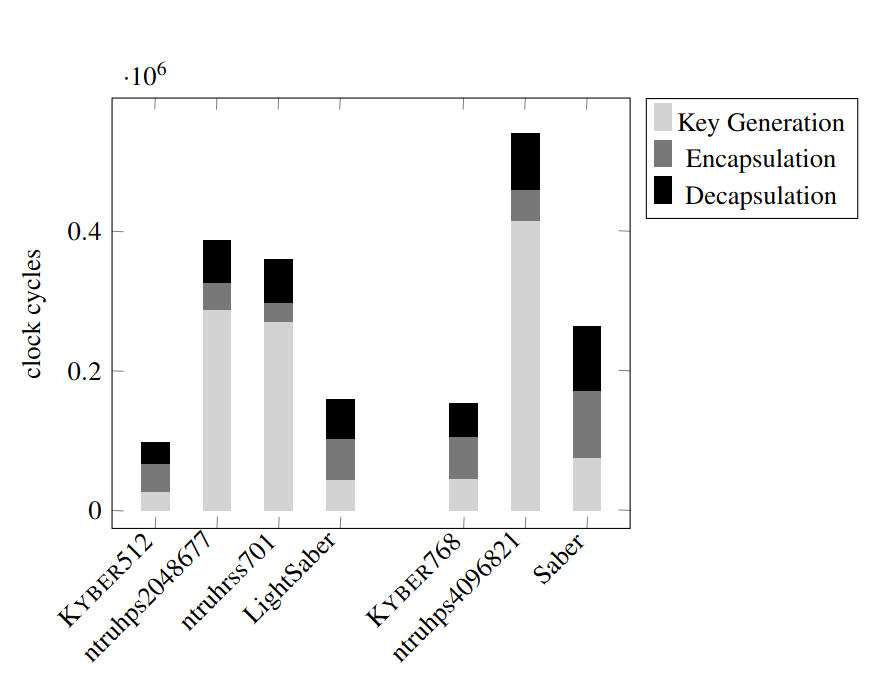
\includegraphics[width=0.75\textwidth]{Figuras/benchmark.png}\\
        \footnotesize{Fonte: Adaptado de \cite{nist_round_3_report}.}
        \label{fig:benchmark}
    \end{figure}
    
    Isso se deve ao fato dos seus cálculos necessitarem principalmente de soma e multiplicação de matrizes e polinômios, que são operações de baixa complexidade. A soma de matrizes e polinômios, por exemplo, possui complexidade $\mathcal{O}(n)$ e a multiplicação matricial $\mathcal{O}(n^2)$. Pelo fato das matrizes serem pequenas, $2 \times 2$, $3 \times 3$ ou $4 \times 4$, dependendo do parâmetro k escolhido, a complexidade do algoritmo em geral é mais afetada pela multiplicação dos elementos dessas matrizes, que no caso são polinômios, e das primitivas criptográficas utilizadas durante os processos (estas primitivas foram removidas deste trabalho para sua simplificação). A multiplicação dos polinômios, pelo fato de pertencerem a um anel quociente, podem ser otimizadas pelo método \ac{NTT}, possuindo assim complexidade logarítmica ao invés de quadrática. Estes fatores de otimização contribuíram significativamente para seu desempenho, e em sua seleção para padronização.